\documentclass[a4paper,12pt]{article}
\usepackage{amsmath}
\usepackage{graphicx}
\usepackage{listings}
\usepackage{caption}
\usepackage{hyperref}
\usepackage{booktabs}
\usepackage{pgfplots} % For including plots
\usepackage{ragged2e}
\usepackage{listings}
\usepackage{float}
\usepackage{geometry}
\usepackage{wrapfig} % Required for wrapping text around figures
\geometry{margin=2.5cm} % <-- Set all margins to 2.5cm. Change as needed.
\usepackage[most]{tcolorbox}

\usepackage{graphicx} % For including images
\usepackage{caption}    % For customized captions
\usepackage{subcaption} % For subfigures (multiple images in one figure environment)
\usepackage{float}      % For more control over float placement, e.g., [H]
% Adjust geometry if needed for better page layout with many images
% \usepackage[margin=2.5cm]{geometry}


\hypersetup{
    hidelinks
}


\usepackage{xcolor}

\definecolor{codegreen}{rgb}{0,0.6,0}
\definecolor{codegray}{rgb}{0.5,0.5,0.5}
\definecolor{codepurple}{rgb}{0.58,0,0.82}
\definecolor{backcolour}{rgb}{0.95,0.95,0.92}

\tcbset{
    frame code={},
    center title,
    left=0pt,
    right=0pt,
    top=0pt,
    bottom=0pt,
    colback=backcolour,
    colframe=white,
    width=\dimexpr\textwidth\relax,
    enlarge left by=0mm,
    boxsep=5pt,
    arc=0pt,outer arc=0pt,
    }



\lstdefinestyle{mystyle}{
    backgroundcolor=\color{backcolour},   
    commentstyle=\color{codegreen},
    keywordstyle=\color{magenta},
    numberstyle=\tiny\color{codegray},
    stringstyle=\color{codepurple},
    basicstyle=\ttfamily\footnotesize,
    breakatwhitespace=false,         
    breaklines=true,                 
    captionpos=b,                    
    keepspaces=true,                 
    numbers=left,                    
    numbersep=5pt,                  
    showspaces=false,                
    showstringspaces=false,
    showtabs=false,                  
    tabsize=2
}

\lstset{style=mystyle}

\usepackage{graphicx} % Required for inserting images

\title{Artificial Intelligence and Machine Learning}
\author{Cliffwalking}
\date{Authors:\\Alessandro Rocchi\\Onorio Iacobelli}

\begin{document}

\maketitle

\tableofcontents

\section{Introduction}
In this Machine Learning project we will focus on the subject of Reinforcement Learning applied to the "Cliff Walking" environment. The goal of the agent is to reach a specified location, by moving in the four directions without falling down the cliff. This problem represents a fundamental challenge in Reinforcement Learning, combining elements of exploration/exploitation tradeoff, temporal credit assignment and policy optimization. This environment provides an excellent testbed for comparing different Reinforcement Learning approaches, in particular tabular Q-learning and Deep Q-Networks (DQN).
\vspace{0,5cm}\\
Our implementation explores both classical tabular methods, suitable for discrete state spaces and modern deep learning approaches that can handle more complex scenarios. Trough extensive experimentation and hyperparameter tuning, we demonstrate how different choices and configurations impact learning performance and convergence behavior. 
\section{Reinforcement Learning}
Reinforcement Learning is a branch of machine learning focused on decision making trough interaction with the environment. Unlike supervised learning, where the correct outputs are given for training, in Reinforcement Learning the agent must discover the optimal behavior by trial and error, guided only by rewards. Formally, Reinforcement Learning is often modeled as a Markov Decision Process (MDP), defined by states, actions, transition probabilities and rewards. The agent's goal is to learn a policy, a mapping from states to actions, that maximizes the expected cumulative reward over time.
\vspace{0,5cm}\\
The core components of a Markov Decision Process are:
\begin{itemize}
    \item \textbf{Agent}: the learner or decision-maker that interacts with the environment. In our case this is the entity navigating the cliff walking grid.
    \item \textbf{Environment}: the external system that the agent interacts with. For cliff walking, this includes the grid world, cliff locations, and reward structure.
    \item \textbf{State (S)}: a representation of the current situation in the environment. In cliff walking, this is the agent's current position in the grid.
    \item \textbf{Action (A)}: the choices available to the agent at any given state.
    \item \textbf{Reward (R)}: the feedback signal from the environment indicating how good or bad the last action was. Rewards guide the learning process.
    \item \textbf{Policy ($\pi$)}: the agent's strategy for choosing actions given states. This can be deterministic (always choose the same action in a given state) or stochastic (choose actions according to a probability distribution).
    \item \textbf{$\delta(s'|s,a)$}: the probability distribution over the transitions.
\end{itemize}
The Reinforcement Learning process follows a continuous loop:
\begin{enumerate}
    \item Observe the current state of the environment
    \item Select an action based on the current policy
    \item Execute the action in the environment
    \item Receive a reward and observe the new state
    \item Update the policy based on the experience
    \item Repeat until learning converges or a stopping criterion is met
\end{enumerate}
One of the fundamental challenges in Reinforcement Learning is balancing \textbf{exploration} (trying new actions to discover potentially better strategies) with \textbf{exploitation} (using knows good actions to maximize rewards). This balancing is crucial because too much exploration can lead to the agent wasting time on suboptimal actions, on the other hand with too little exploration the agent may get stuck in a local optimum and never discover the best strategy.
\subsection{Q-Learning}
Q-Learning is a model-free Reinforcement Learning algorithm that learns the quality of actions, telling the agent what actions to take under what circumstances. The "Q" stands for quality, representing the expected future reward for taking a specific action in a specific state.\\ The \textbf{Q-function} Q(s,a) represents the expected cumulative reward when taking action 'a' in state 's' and then following the optimal policy. The learning process involves iteratively updating these Q-values using the Bellman equation:
\begin{figure}[H]
    \centering
    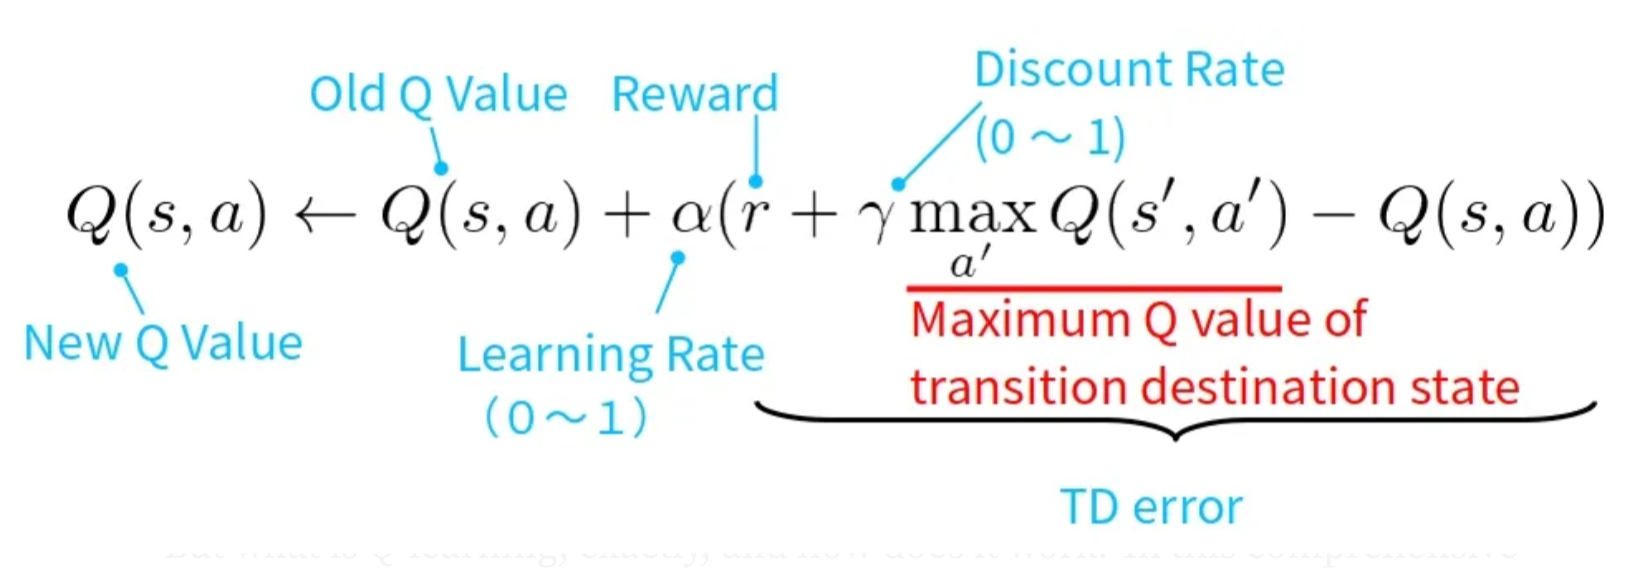
\includegraphics[scale=0.5]{bellman.png}
\end{figure}
Where:
\begin{itemize}
    \item \textbf{$\alpha$ (alpha)}: learning rate controlling how quickly new information overrides old information
    \item \textbf{r}: immediate reward received
    \item \textbf{$\gamma$ (gamma)}: discount factor determining the importance of future rewards
    \item \textbf{s'}: next state after taking action 'a' in state 's'
\end{itemize}
\textbf{Tabular Q-Learning} maintains explicit Q-values for every (state, actions) pair in a lookup table. This approach works well for environments with small, discrete state and action spaces but becomes impractical as the state space grows.
\vspace{0,5cm}\\
\textbf{Deep Q-Networks (DQN)} use neural networks to approximate the Q-function, enabling the handling of large or continuous state spaces. Instead of storing individual Q-values, the network learns to map states to Q-values for all possible actions.
\vspace{0,5cm}\\
To balance exploration and exploitation, we implement an epsilon-greedy policy:
\begin{itemize}
    \item With probability \textbf{$\varepsilon$ (epsilon)}: choose a random action (exploration)
    \item With probability \textbf{(1-$\varepsilon$)}: choose the action with the highest Q-value (exploitation)
\end{itemize}
The epsilon value starts high (encouraging exploration) and gradually decreases (shifting toward exploitation) as learning progresses.
\section{Environment}
The Cliff Walking environment is part of the Toy Text environments which contains general information about the environment. It involves crossing a grid world from start to goal while avoiding falling off a cliff.
\begin{figure}[H]
    \centering
    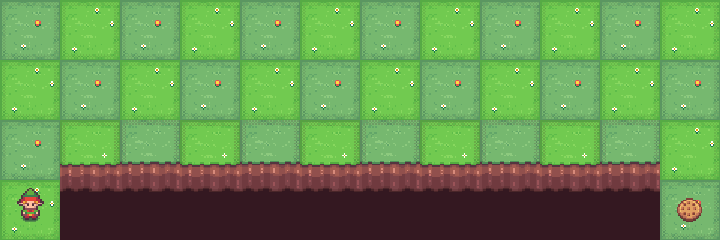
\includegraphics[scale=0.7]{cliff_walking.png}
\end{figure}
\subsection{Description}
The game starts with the player at location [3, 0] of the 4x12 grid world with the goal located at [3, 11]. If the player reaches the goal the episode ends.
\vspace{0,5cm}\\
A cliff runs along [3, 1..10]. If the player moves to a cliff location it returns to the start location.
\vspace{0,5cm}\\
The player makes moves until they reach the goal.
\subsection{Action Space}
The action shape is (1,) in the range \{0, 3\} indicating which direction to move the player.
\begin{itemize}
    \item 0: Move up
    \item 1: Move right
    \item 2: Move down
    \item 3: Move left
\end{itemize}
Actions that would move the agent outside the grid boundaries result in no movement (the agent stays in the same position).
\subsection{Observation Space}
There are 3 x 12 + 1 possible states. The player cannot be at the cliff, nor at the goal as the latter results in the end of the episode. What remains are all the positions of the first 3 rows plus the bottom-left cell.
\vspace{0,5cm}\\
The observation is a value representing the player’s current position as current\_row * ncols + current\_col (where both the row and col start at 0).\\For example, the starting position can be calculated as follows: 3 * 12 + 0 = 36.
\vspace{0,5cm}\\
The observation is returned as an int().
\subsection{Reward}
The reward system is designed to encourage finding the shortest safe path while severely penalizing dangerous moves:
\begin{itemize}
    \item \textbf{Standard step}: -1 reward (encourages shorter paths)
    \item \textbf{Falling off cliff}: -100 reward + episode termination
    \item \textbf{Reaching goal}: 0 reward + episode termination
\end{itemize}
This reward structure creates an interesting dilemma: the shortest path (along the cliff edge) is risky but potentially more rewarding if executed perfectly, while the safe path (around the cliff) is longer but more reliable.
\vspace{0,5cm}\\
The episode terminates when the Agent reaches the goal position, falls of the cliff or the episode can exceeds maximum step limit.
\section{Implementation}
Our approach to solving the Cliff Walking problem implements and compares two fundamental reinforcement learning methodologies: Tabular Q-Learning and Deep Q-Networks (DQN). This comparison allows us to understand the strengths and limitations of each approach while demonstrating how different choices affect learning performance.
\vspace{0,5cm}\\
Both implementations use the code Q-Learning update rule, which is an off-policy temporal difference learning method.
$$Q(s,a) \leftarrow Q(s,a) + \alpha \big[r + \gamma \max_{a'} Q(s',a') - Q(s,a)\big]$$
This update rule is off-policy, meaning it learns about the optimal policy while following a potentially different policy (epsilon-greedy). This property makes Q-learning robust and widely applicable.
\subsection{Framework}
Our solution utilizes the following Python libraries:
\begin{itemize}
    \item \textbf{Gymnasium}: standard Reinforcement Learning environment interface
    \item \textbf{NumPy}: efficient numerical computations for tabular methods
    \item \textbf{PyTorch}: deep learning framework for DQN implementation
    \item \textbf{Matplotlib}: visualization of learning curves and performance metrics
\end{itemize}
The modular design allows easy experimentation with different hyperparameters and direct comparison between approaches under identical conditions.
\subsection{Tabular Q-Learning Implementation Details}
The algorithm follows the standard Q-Learning approach but is tailored for the Cliff Walking environment.
\subsubsection{Initialize Q-table}
The Q-table is initialized with zeros. Its shape corresponds to the number of state and the number of possible actions in the environment:
\begin{lstlisting}
    n_states = env.observation_space.n
    n_actions = env.action_space.n
    Q = np.zeros((n_states, n_actions))
\end{lstlisting}
\subsubsection{Training Loop}
For each episode, the environment is reset and the agent interacts with it until termination.
\subsubsection{Action Selection ($\varepsilon$-greedy)}
The agent chooses an action using the $\varepsilon$-greedy strategy: with probability $\varepsilon$ it selects a random action (exploration), and otherwise it selects the action with the highest Q-value (exploitation).
\begin{lstlisting}
    if np.random.rand() < epsilon:
        action = env.action_space.sample()
    else:
        action = np.argmax(Q[state])
\end{lstlisting}
\subsubsection{Environment Step and Q-value Update}
After takin an action, the agent observes the next state and reward. The Q-value is updated using the Temporal Difference (TD) learning rule:
\begin{lstlisting}
    old_value = Q[state, action]
    best_next = np.max(Q[next_state])
    td_target = reward + gamma * best_next * (not done)
    td_error = td_target - old_value
    Q[state, action] += alpha * td_error
\end{lstlisting}
\subsubsection{Track Metrics}
During the training, the following metrics are stored for later visualization:
\begin{itemize}
    \item Episode reward: cumulative sum of the rewards per episode
    \item Epsilon: exploration rate over time
    \item TD errors: average temporal-difference errors per episode
\end{itemize}
\subsubsection{Epsilon Decay}
At the end of each episode, epsilon is decayed to gradually shift from exploration to exploitation:
\begin{lstlisting}
    epsilon = max(min_epsilon, epsilon * epsilon_decay)
\end{lstlisting}
\subsection{Deep Q-Network (DQN) Implementation}
Our DQN implementation uses a neural network to approximate Q-values, enabling more complex function approximation capabilities. The network architecture is configurable trough hyperparameters.
\subsubsection{Network Architecture}
\begin{lstlisting}
    class DQN(nn.Module):
    def __init__(self, state_size, action_size):
        super().__init__()
        self.embedding = nn.Embedding(state_size, 16)
        
        layers = []
        input_size = 16
        for _ in range(DQN_HIDDEN_LAYERS):
            layers.append(nn.Linear(input_size, DQN_NODES_PER_LAYER))
            layers.append(nn.ReLU())
            input_size = DQN_NODES_PER_LAYER
            
        layers.append(nn.Linear(input_size, action_size))
        self.net = nn.Sequential(*layers)
    
    def forward(self, x):
        x = self.embedding(x)
        return self.net(x)
\end{lstlisting}
\begin{itemize}
    \item \textbf{State Embedding}: 16-dimensional embedding layer converts discrete states to dense representations
    \item \textbf{Configurable Depth}: number of hidden layers determined by hyperparameters
    \item \textbf{ReLU Activation}: non-linear activation functions enabling complex function approximation
    \item \textbf{Output Layer}: linear layer producing Q-values dor all actions
\end{itemize}
DQN incorporates Experience Replay Buffer to break temporal correlations and improve sample efficiency:
\begin{lstlisting}
    replay_buffer = deque(maxlen=10_000)

    # Store experiences
    replay_buffer.append((state, action, reward, next_state, done))

    # Sample random batch for training
    if len(replay_buffer) >= batch_size:
        batch = random.sample(replay_buffer, batch_size)
        # Process batch for network update
\end{lstlisting}
Benefits of Experience Replay:
\begin{itemize}
    \item \textbf{Decorrelated Updates}: reduces harmful correlation between consecutive experiences 
    \item \textbf{Sample Efficiency}: reuses experiences multiple times for training
    \item Stable Learning: smoother gradient updates trough diverse batch sampling
\end{itemize}
\begin{lstlisting}
    policy_net = DQN(n_states, n_actions)  # Updated every step
    target_net = DQN(n_states, n_actions)  # Updated periodically
    
    # Target network update
    if episode % target_update_freq == 0:
        target_net.load_state_dict(policy_net.state_dict())
\end{lstlisting}
Target Network Purpose:
\begin{itemize}
    \item \textbf{Stable Targets}: reduces moving target problem in Q-learning
    \item \textbf{Reduced Correlation}: separates action selection from target value computation
    \item \textbf{Improved Convergence}: more stable learning dynamics
\end{itemize}
Our implementation includes a comprehensive configuration system enabling systematic experimentation:
\begin{lstlisting}
    # Configuration parameters
    DQN_HIDDEN_LAYERS = 2
    DQN_NODES_PER_LAYER = 128
    DQN_BATCH_SIZE = 64
    DQN_GAMMA = 0.99
    DQN_EPSILON_DECAY = 0.995
    DQN_TARGET_UPDATE_FREQ = 10
\end{lstlisting}
\section{Evaluation Framework}
Both algorithms share a common evaluation framework ensuring fair comparison:
\begin{lstlisting}
    def evaluate_agent(env, policy_net=None, Q=None, tabular=True, episodes=1000):
    successes, falls, total_rewards = 0, 0, []
    
    for _ in range(episodes):
        state, _ = env.reset()
        done, ep_reward = False, 0
        
        while not done:
            if tabular:
                action = np.argmax(Q[state])
            else:
                with torch.no_grad():
                    action = policy_net(state_tensor).argmax().item()
            
            next_state, reward, terminated, truncated, _ = env.step(action)
            done = terminated or truncated
            ep_reward += reward
            
            if reward == -100:  # Cliff fall detection
                falls += 1
            if done and next_state == (env.observation_space.n - 1):
                successes += 1
                
    return successes, falls, total_rewards
\end{lstlisting}
Evaluation Metrics:
\begin{itemize}
    \item \textbf{Success Rate}: percentage of episodes reaching the goal
    \item \textbf{Cliff Falls}: number of cliff accidents
    \item \textbf{Average Reward}: mean cumulative reward per episode
    \item \textbf{Average Steps}: mean episodes length, indicating path efficiency
\end{itemize}
\section{Results}
\end{document}